\documentclass[]{standalone}

\usepackage{adjustbox}

\usepackage{amsmath}
\usepackage{xfrac}
\usepackage{mathrsfs}

\usepackage{circuitikz}
\usepackage{tikz}
\usetikzlibrary{arrows, patterns, decorations.pathmorphing, backgrounds, positioning, fit, petri, shapes, trees, matrix, chains, decorations, decorations.pathreplacing, decorations.fractals, calc,snakes,trees, decorations.markings}

\usepackage{color}
\definecolor{soton}{RGB}{7,51,71}
\colorlet{comms}{red!50!yellow}
\colorlet{payld}{pink!50!purple}
\colorlet{obdh}{green!50!black}

\begin{document}

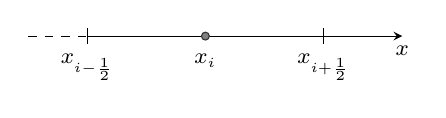
\begin{tikzpicture}

\draw[dashed] (-0.75,0) -- (0, 0);
\draw[-stealth] (0,0) -- (4,0) node[below] {\footnotesize{$x$}};
\draw (0,0.1) -- (0, -0.1) node[below] {\footnotesize{$x$}\tiny{$_{i-\tfrac{1}{2}}$}};
\draw (3,0.1) -- (3, -0.1) node[below] {\footnotesize{$x$}\tiny{$_{i+\tfrac{1}{2}}$}};
\node[below] at (1.5, -0.1) {\footnotesize{$x$}\tiny{$_{i}$}};
\draw[black!80, fill=black!50] (1.5, 0) circle (0.05);

\end{tikzpicture}


\end{document}